%------------------------------------------------------------------------------
% Document Header
%------------------------------------------------------------------------------
\documentclass[10pt]{beamer}

\usetheme{metropolis}
\usepackage{appendixnumberbeamer}

\usepackage{booktabs}
\usepackage[scale=2]{ccicons}

\usepackage{pgfplots}
\usepgfplotslibrary{dateplot}

\usepackage{xspace}
\newcommand{\themename}{\textbf{\textsc{metropolis}}\xspace}

\usepackage{url}
\usepackage{courier}
\usepackage[skip=5pt]{caption}
\usepackage{xcolor}
\usepackage{framed}
\usepackage{float}
\usepackage{listings}

\definecolor{groovyblue}{HTML}{0000A0}
\definecolor{groovygreen}{HTML}{008000}
\definecolor{regexcolor}{HTML}{003300}
\definecolor{comment}{HTML}{B22400}
\definecolor{functions}{HTML}{660000}

\lstdefinelanguage{Groovy}[]{Java}{
  basicstyle=\ttfamily,
  columns=fixed,
  keywords=[3]{def, new, as, in, use, each, grep, inject, INVASIVE, CANCER, LOBULAR, DUCTAL, \$A, \$N},
  keywords=[4]{select, create, match, process, code, text},
  keywords=[5]{Sentence, CancerFinding, PostNegationTerm, PreNegationTerm, DictMatch, Token, AnnotationRegex, HistoryTerm},
  keywordstyle=[3]\bfseries,
  keywordstyle=[4]\color{functions}\bfseries,
  keywordstyle=[5]\color{groovyblue}\bfseries,
  stringstyle=\color{groovygreen}\ttfamily,
  commentstyle=\color{comment},
  moredelim=[is][\textcolor{groovyblue}]{\%\%}{\%\%},
  xleftmargin=0em,
  literate={~} {$\sim$}{1},
  aboveskip=0pt,
  belowskip=-5pt
}
\lstset{language=Groovy}

\newcommand{\DSLAnnotator}{\texttt{DSL\_Annotator}}

\title{Information Extraction}
\subtitle{Regular Expressions and Beyond}
\date{February 22, 2019}
\author{Will Thompson, Ph.D.}
%------------------------------------------------------------------------------

%------------------------------------------------------------------------------
% Document Body
%------------------------------------------------------------------------------
\begin{document}
\maketitle

%------------------------------------------------------------------------------
\begin{frame}{Table of contents}
  \setbeamertemplate{section in toc}[sections numbered]
  \tableofcontents[hideallsubsections]
\end{frame}
%------------------------------------------------------------------------------

%------------------------------------------------------------------------------
\section{Introduction}
%------------------------------------------------------------------------------

%------------------------------------------------------------------------------
\begin{frame}[fragile]{Natural Language Processing: Use Cases}
  Some practical use cases for NLP:
  \begin{itemize}
    \item Text exploration (keyphrases, topic models)
    \item Text classification (including sentiment analysis)
    \item \alert{Information Extraction (unstructured $\rightarrow$ structured)}
  \end{itemize}
\end{frame}
%------------------------------------------------------------------------------

%-----------------------------------------------------------------------------
\begin{frame}{Unstructured Data}
  \begin{columns}
    \begin{column}{0.5\textwidth}
      Vast quantities of information are encoded as \alert{unstructured data}, in the form of natural language text.
      \\ \vspace{2em}
      But it can be hard to make this information available for computational analysis at scale.
    \end{column}
    \begin{column}{0.5\textwidth}
      \begin{center}
        \fbox{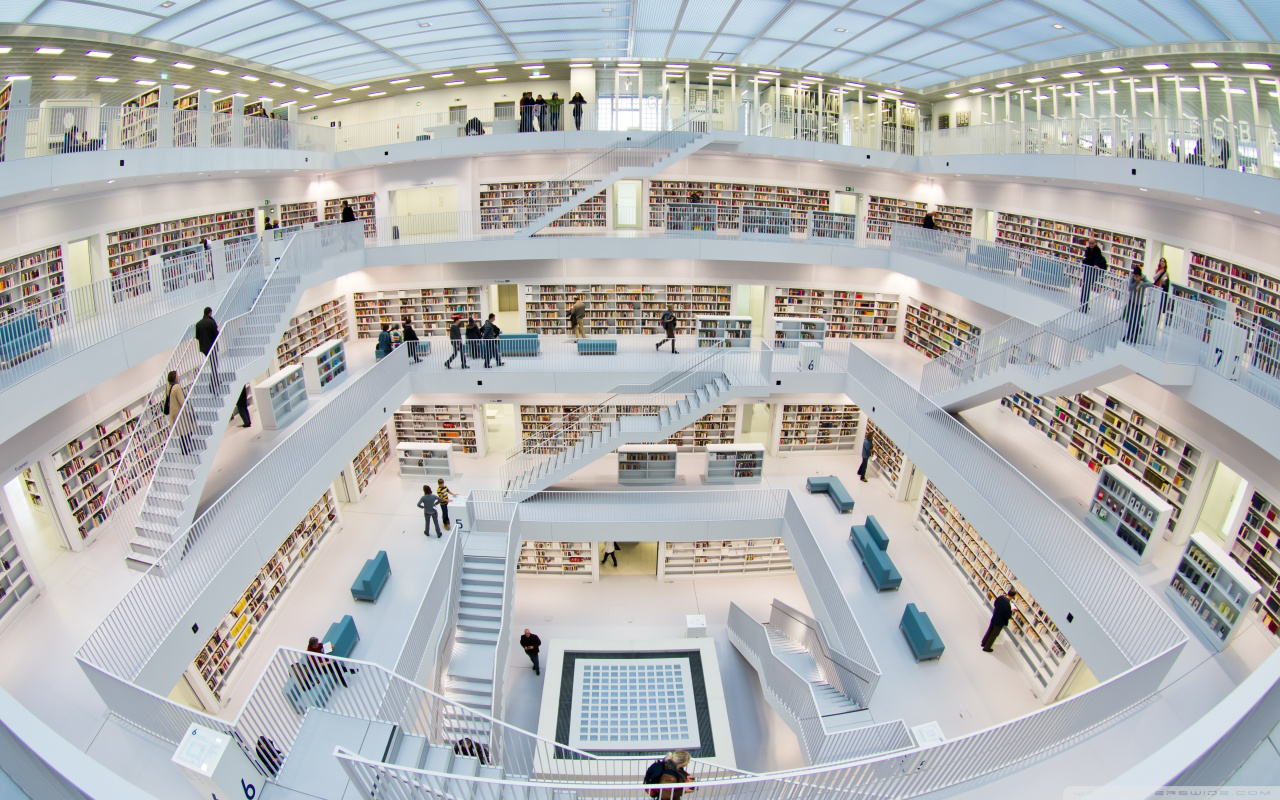
\includegraphics[scale=0.12]{figures/library.png}}
      \end{center}
    \end{column}
  \end{columns}
\end{frame}
%-----------------------------------------------------------------------------

%-----------------------------------------------------------------------------
\begin{frame}{Unstructured Data}
\begin{columns}
\begin{column}{0.4\textwidth}
  What a \alert{human} sees:
  \\ \vspace{5em}
  What a \alert{computer} sees:
\end{column}
\begin{column}{0.6\textwidth}
\begin{center}
  \fbox{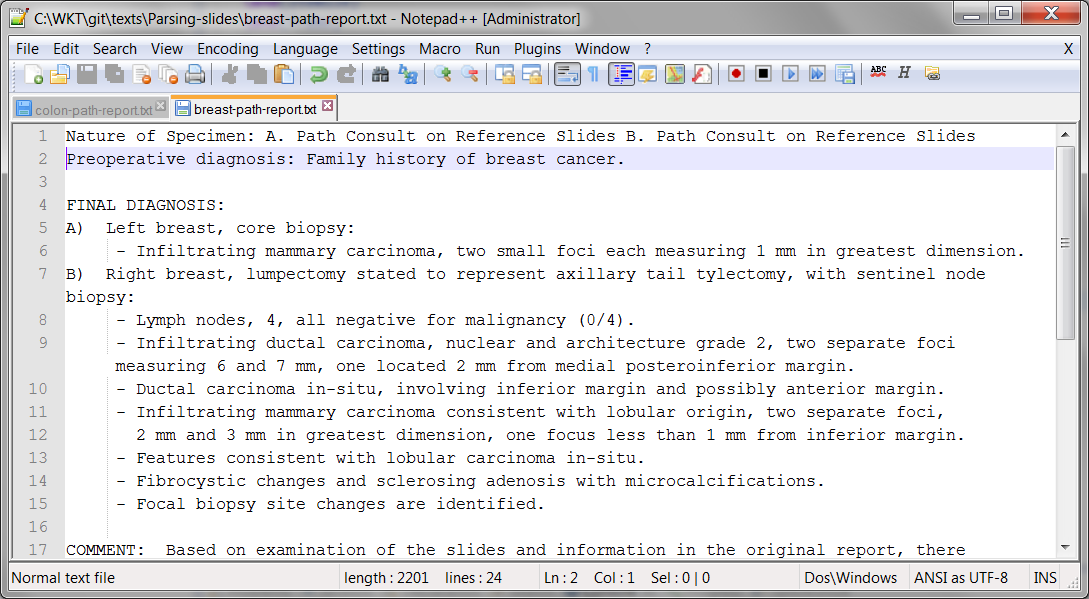
\includegraphics[scale=0.16]{figures/breast-cancer-note-screenshot.png}}
  \\ \vspace{1em}
  \fbox{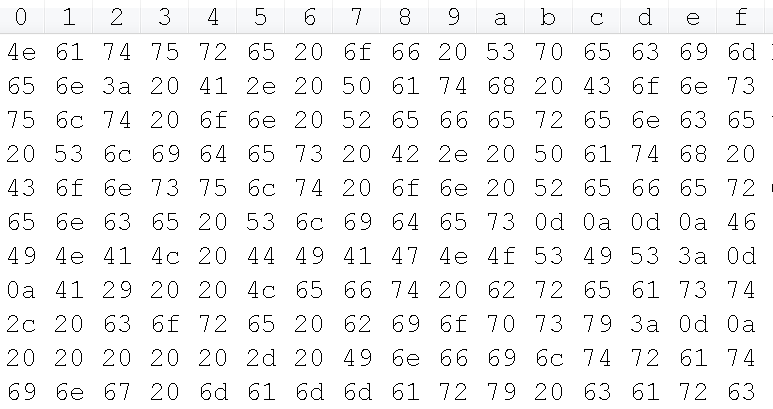
\includegraphics[scale=0.22]{figures/breast-cancer-note-screenshot-hex.png}}
\end{center}
\end{column}
\end{columns}
\end{frame}
%-----------------------------------------------------------------------------

%------------------------------------------------------------------------------
\begin{frame}{Information Extraction}

Information extraction (IE) can be used to convert some of the information stored in text into \alert{structured data}:

\begin{enumerate}
   \item Search for relevant chunks of information in a corpus
   \item Map these chunks to structured representations (potentially including relationships)
   \item Store the results in structured format for downstream analysis
\end{enumerate}

\begin{center}
	\fbox{
\includegraphics[scale=0.4]{figures/unstructured.png}}
\end{center}

\end{frame}
%------------------------------------------------------------------------------
%------------------------------------------------------------------------------
\begin{frame}{Example Use Case}
  \begin{center}
    \fbox{
\includegraphics[scale=0.5]{figures/official-register.png}}
  \end{center}
\end{frame}
%------------------------------------------------------------------------------

%------------------------------------------------------------------------------
\begin{frame}{Example Use Case}
  \begin{center}
    \fbox{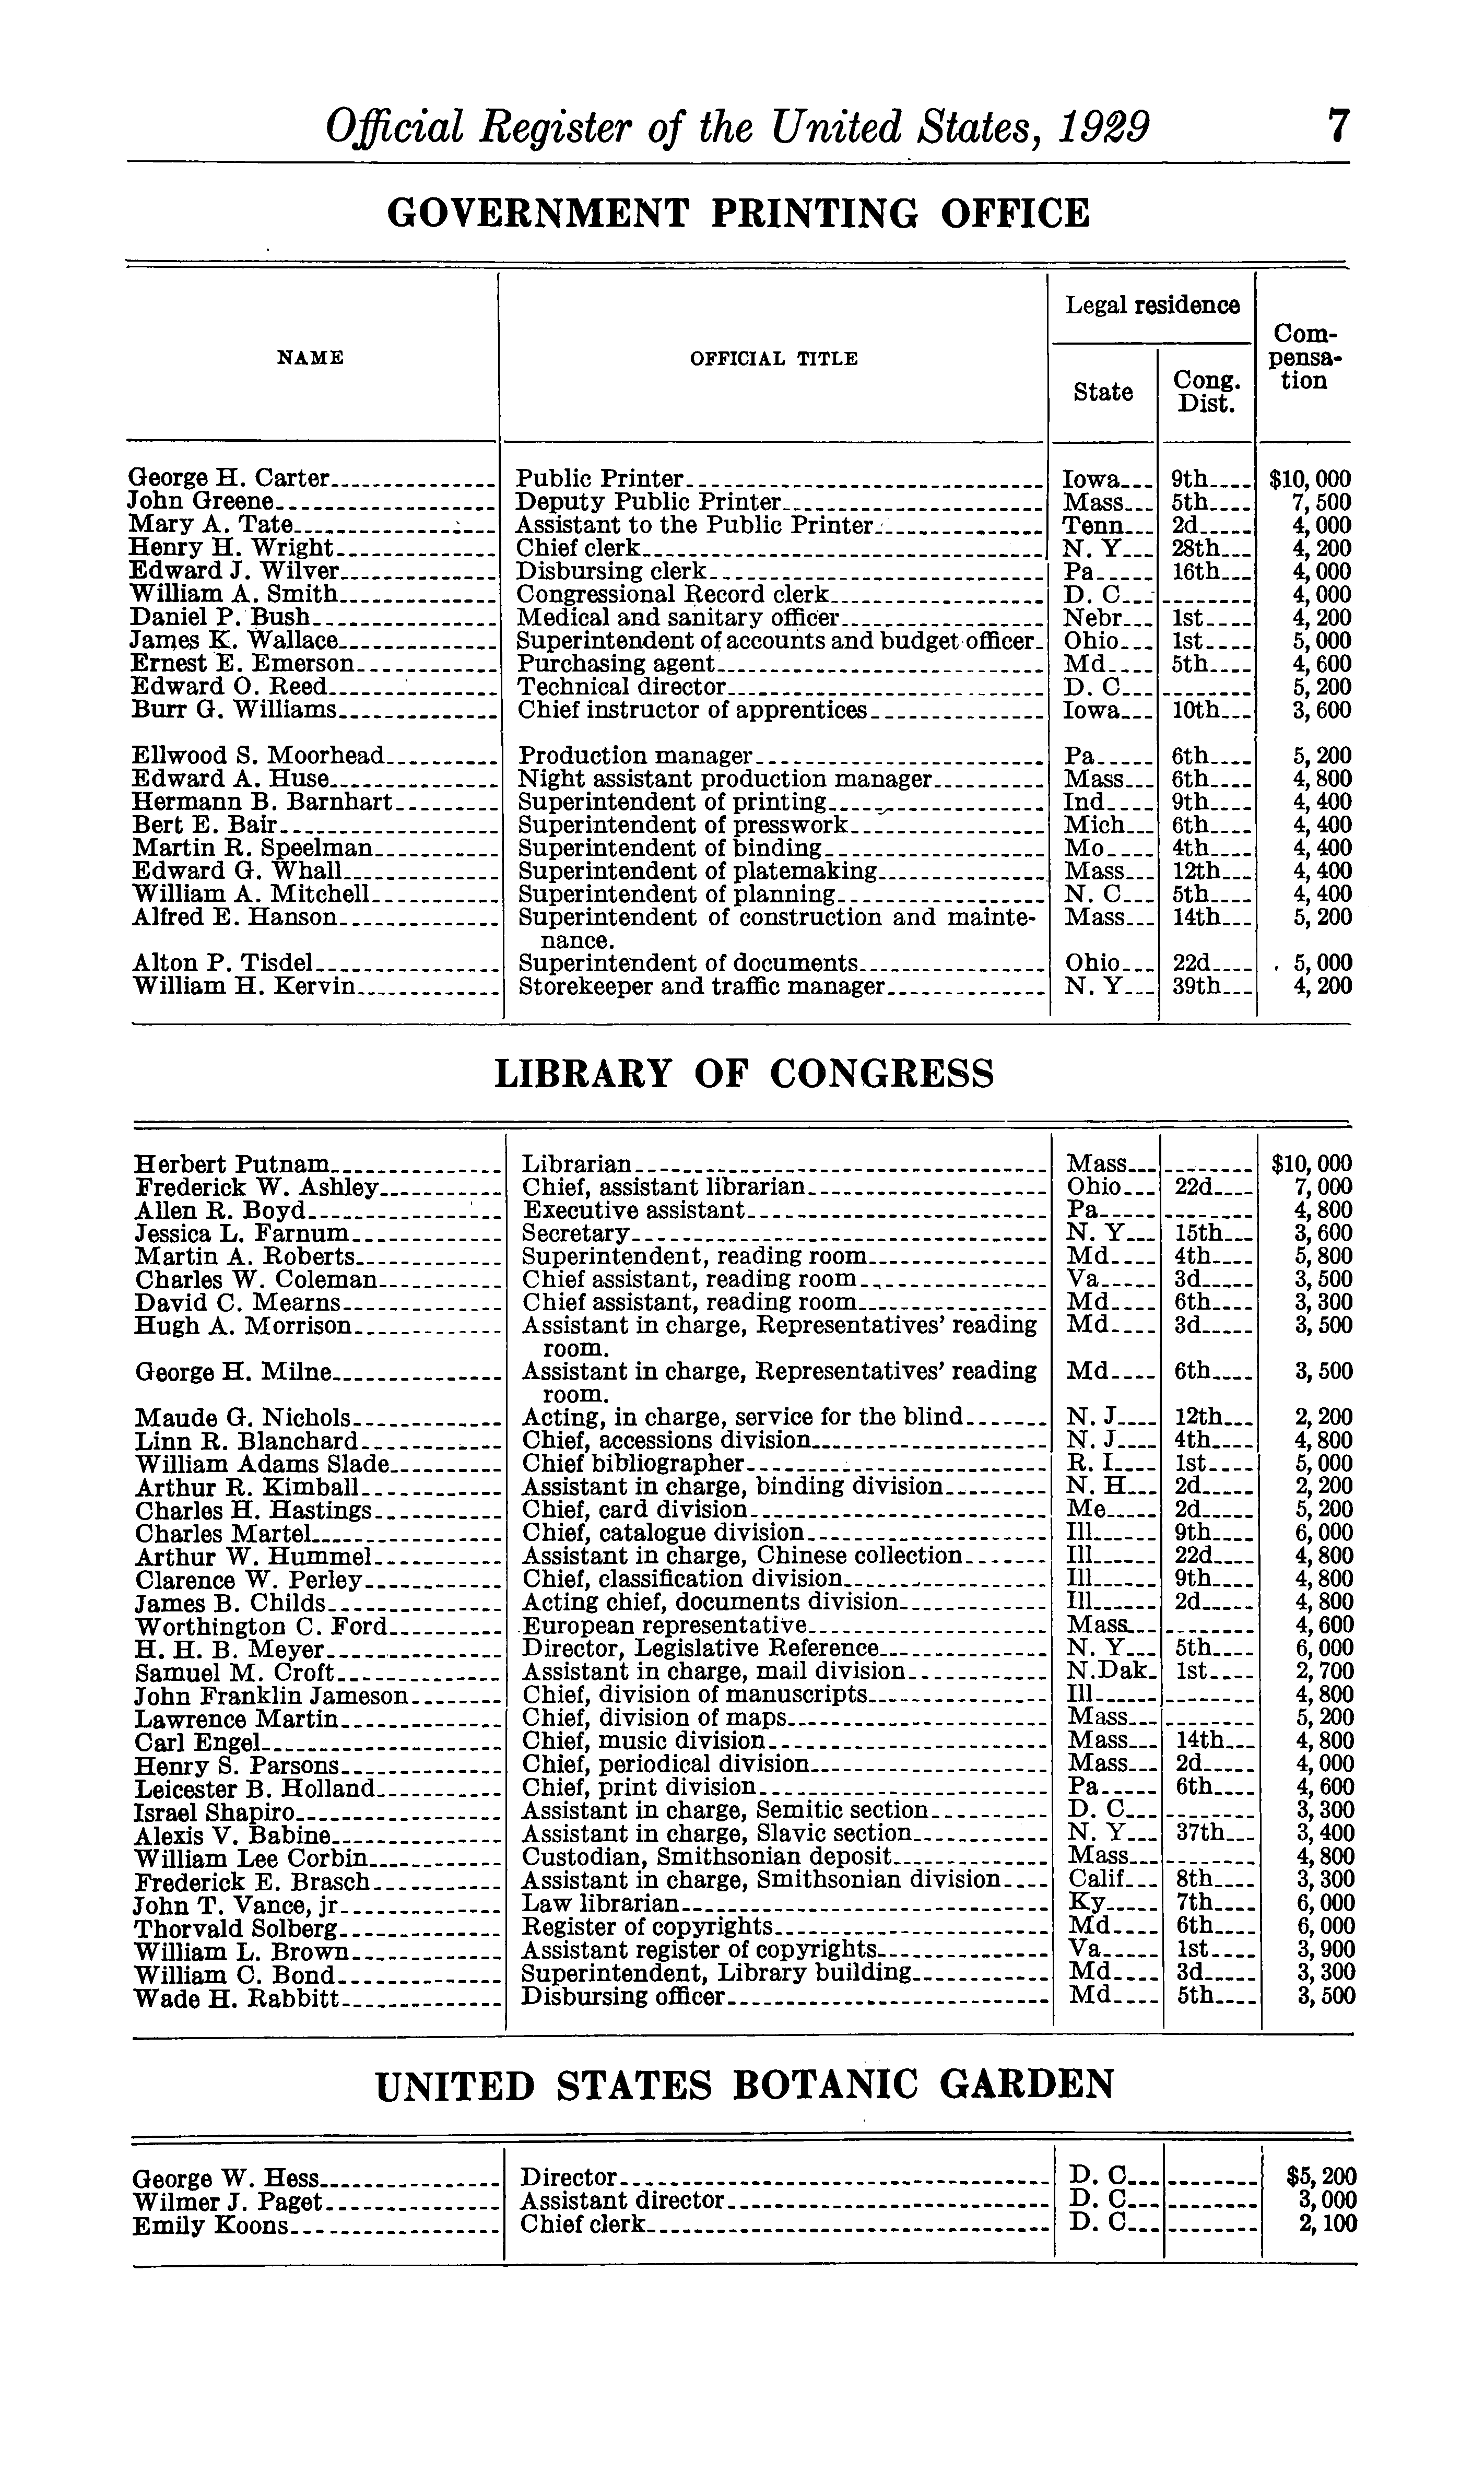
\includegraphics[scale=0.1]{figures/excerpt-p17.png}}
  \end{center}
\end{frame}
%------------------------------------------------------------------------------

%------------------------------------------------------------------------------
\section{Regular Expressions}
%------------------------------------------------------------------------------

%------------------------------------------------------------------------------
\begin{frame}{Regular Expressions}
\begin{itemize}
  \item \alert{Regular expressions} (RE) are a compact and expressive mini-language for defining \alert{patterns} over text
  \item RE functionality is available in most modern programming languages
  \item RE core features include:
  \begin{itemize}
    \item Sequences: \texttt{/pneumonia/}
    \item Disjunction: \texttt{/(a|b|c)/}
    \item Ranges: \texttt{/[A-Z]/}, \texttt{/[0-9]/}
    \item Repetition: \texttt{/[A-Z]*/}, \texttt{/[0-9]+/}
    \item Optionality: \texttt{/[Cc]olou?r/}
  \end{itemize}
  \item \textcolor{blue}{\url{http://web.stanford.edu/~jurafsky/slp3}}
\end{itemize}
\end{frame}
%------------------------------------------------------------------------------

%------------------------------------------------------------------------------
\begin{frame}{Regex: Formal Language Theory}
  \begin{center}
    \fbox{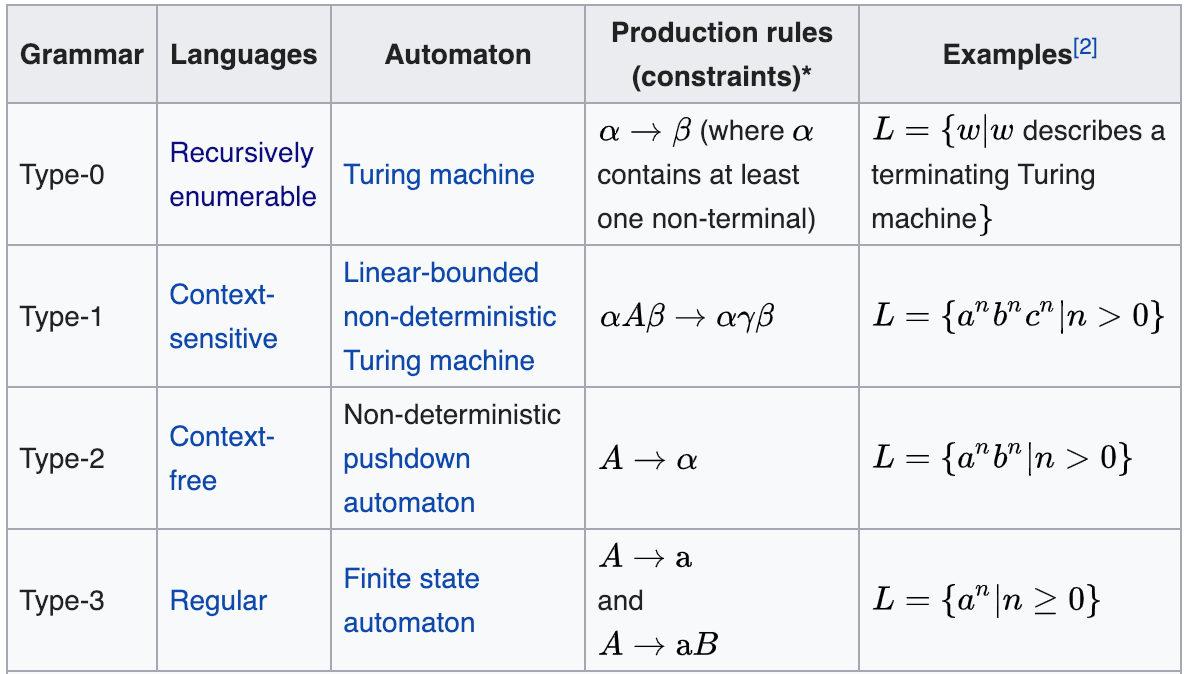
\includegraphics[scale=0.4]{figures/chomsky-hierarchy.png}}
  \end{center}
  \alert{Regular Expressions} $\equiv$ \alert{Regular Languages} $\equiv$ \alert{Finite State Machines}
\end{frame}
%------------------------------------------------------------------------------

%------------------------------------------------------------------------------
\begin{frame}{Finite State Machines}
  \begin{center}
    \fbox{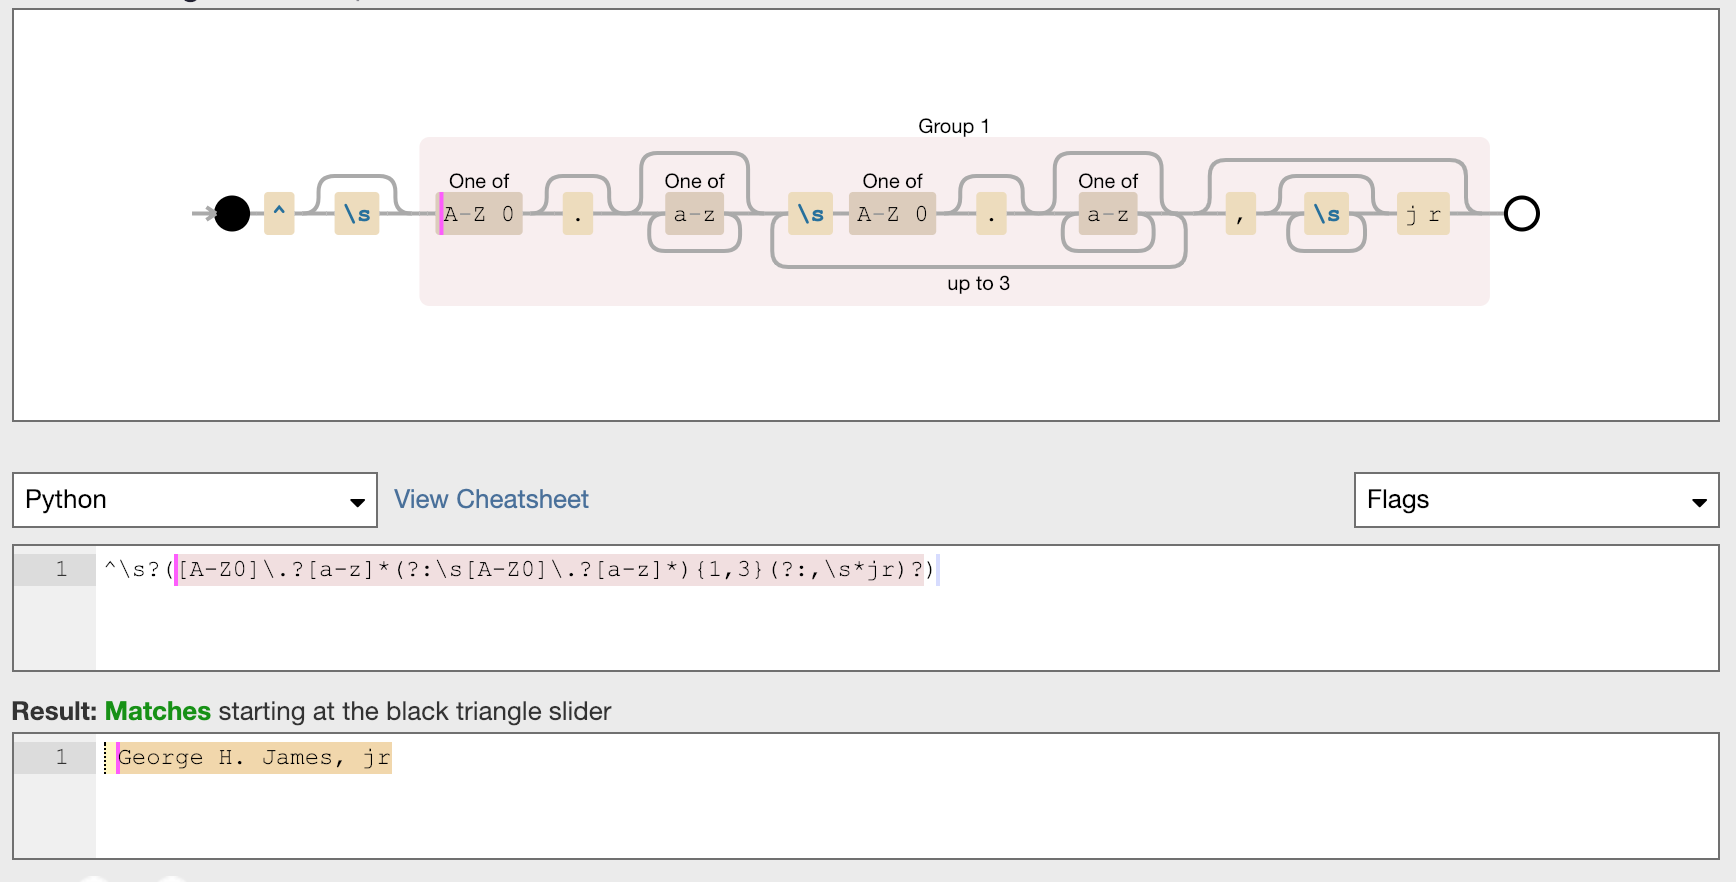
\includegraphics[scale=0.3]{figures/finite-state-machine.png}}
  \end{center}
  \begin{center}
    \textcolor{blue}{\url{https://www.debuggex.com/}}
  \end{center}
\end{frame}
%------------------------------------------------------------------------------

%------------------------------------------------------------------------------
\begin{frame}[fragile]{Demo: Developing Regular Expressions}

\begin{center}
  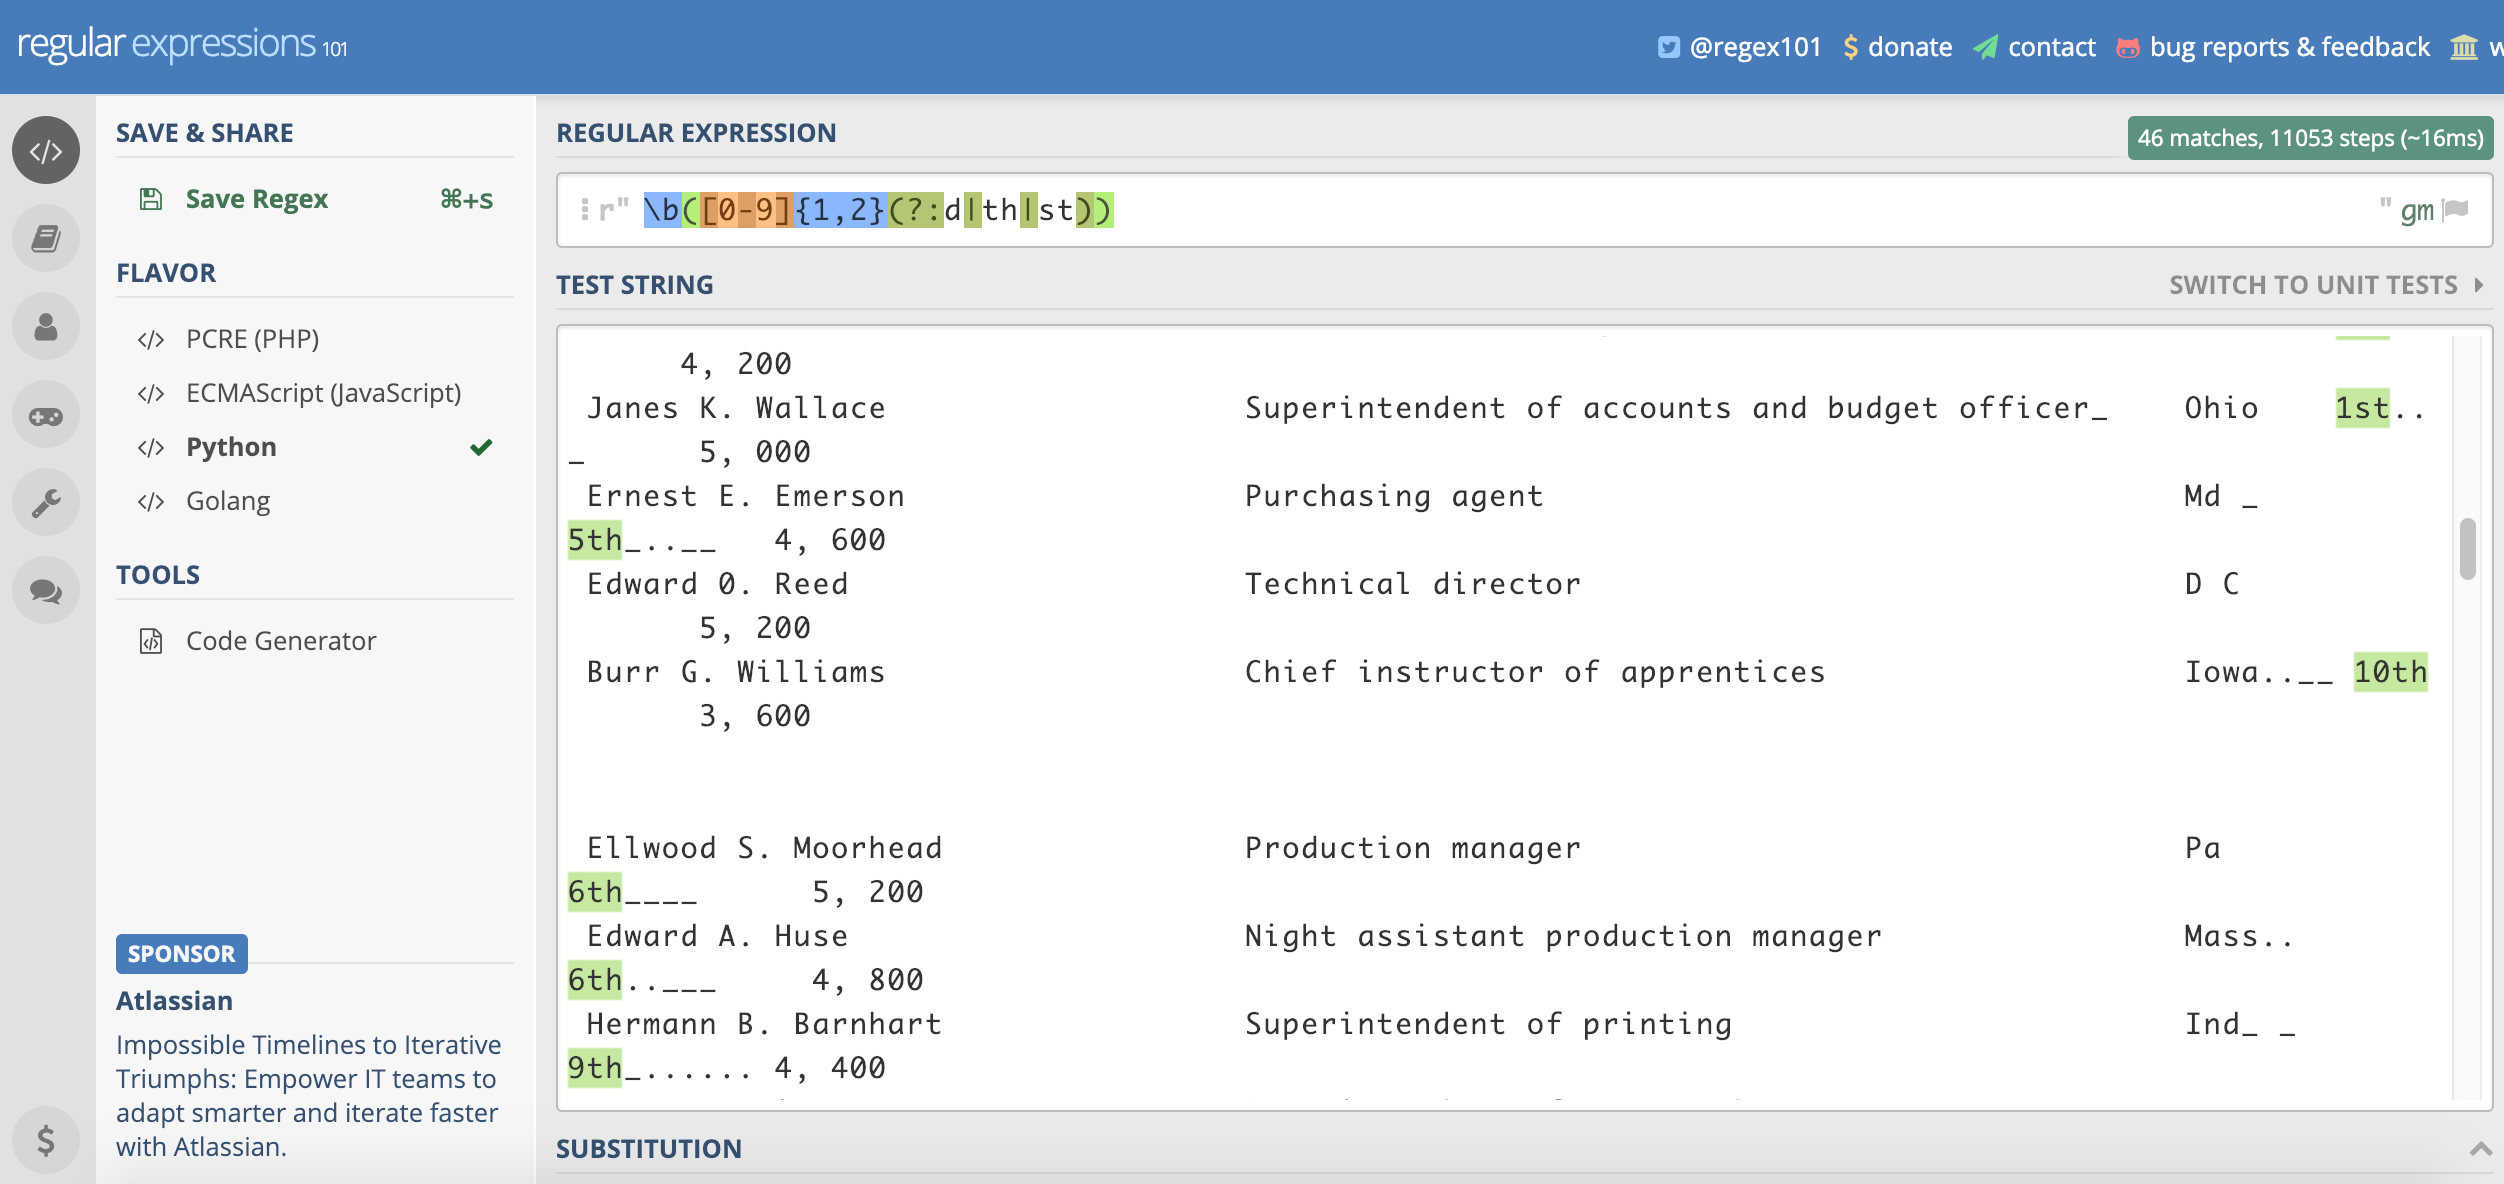
\includegraphics[scale=0.25]{figures/regex101-screenshot.png}
  \\ \vspace{1em}
  \textcolor{blue}{\url{https://regex101.com/}}
  \\
  (For fun: \textcolor{blue}{\url{https://regexcrossword.com/}})
\end{center}

\end{frame}
%------------------------------------------------------------------------------

%------------------------------------------------------------------------------
\begin{frame}[fragile]{Demo: Complete Working Example}
  \begin{center}
    \fbox{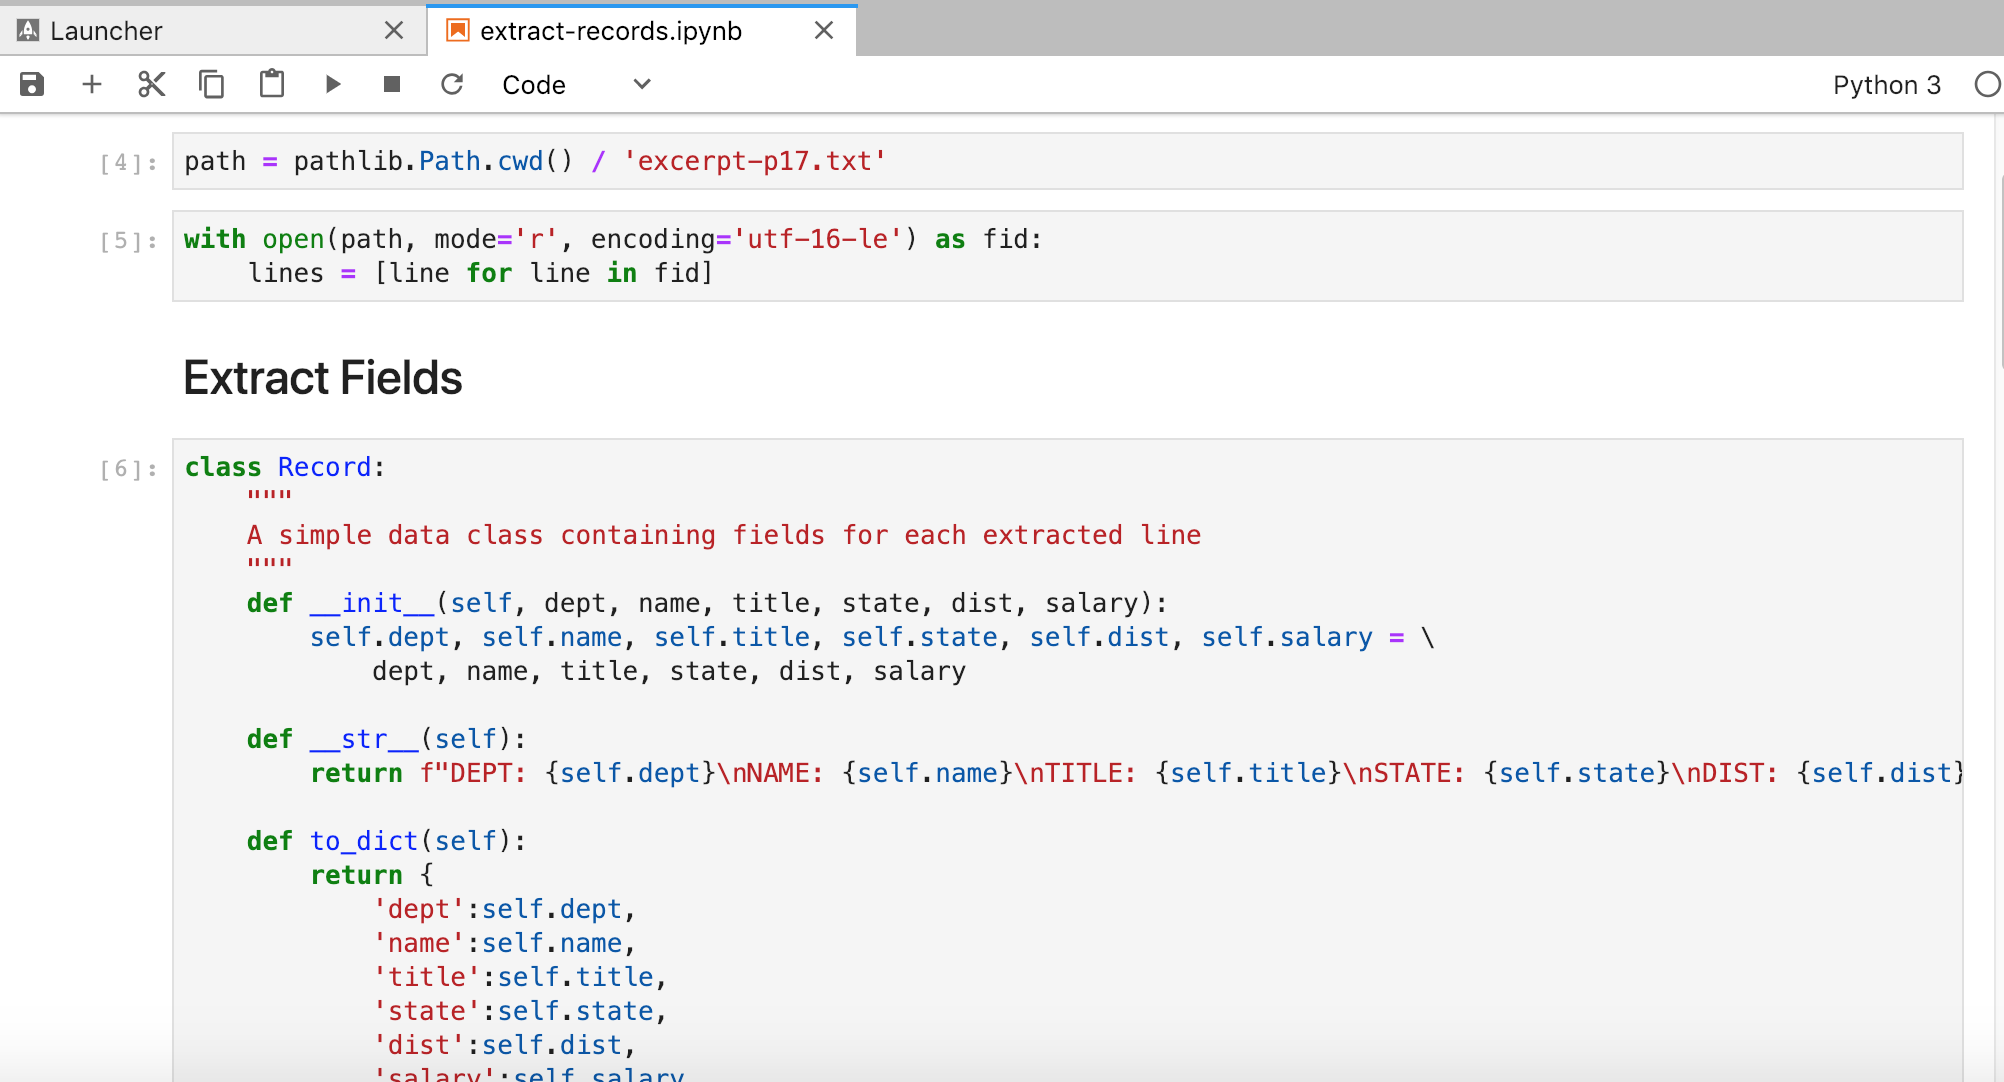
\includegraphics[width=0.9\textwidth]{figures/jupyter-notebook-screenshot.png}}
  \end{center}
\end{frame}
%------------------------------------------------------------------------------

%------------------------------------------------------------------------------
\begin{frame}{Evaluating Performance}
\begin{tabular}{p{5cm} p{7cm}}
    \vspace{0pt}
    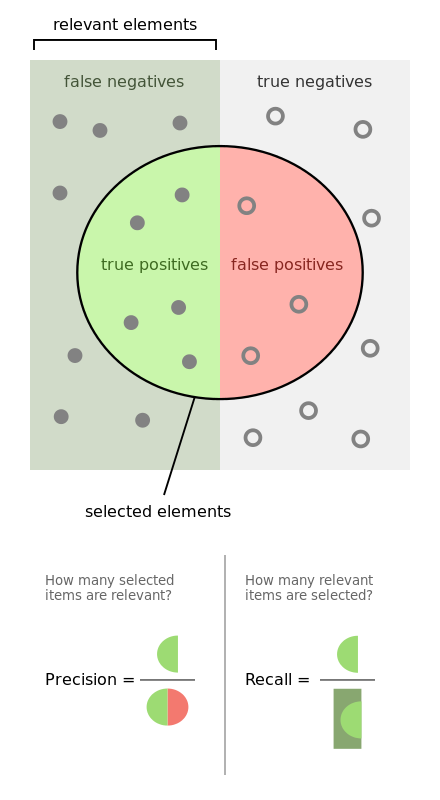
\includegraphics[width=0.4\textwidth]{figures/precisionrecall.png}
    &
    \vspace{0pt}
    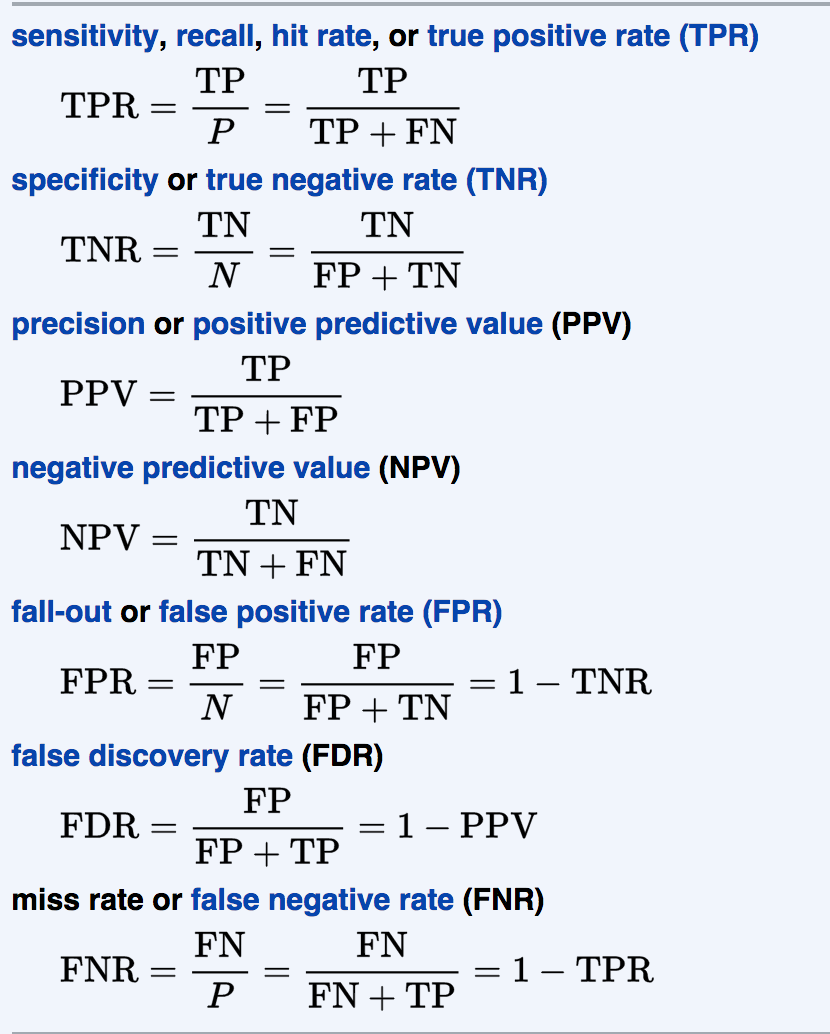
\includegraphics[width=0.5\textwidth]{figures/precisionrecall-formulas.png}
\end{tabular}
\end{frame}
%------------------------------------------------------------------------------

%------------------------------------------------------------------------------
\begin{frame}[fragile]{Annotation Pattern Matching}

\begin{lstlisting}[frame=single]
def regex = new AnnotationRegex(
 (DictMatch, [code:INVASIVE])
 (DictMatch, [code:CANCER])
 ( (Token, [text:/with|having|/])(0,1)
   (DictMatch, [code:LOBULAR|DUCTAL)
   (Token, [text:/features/]) )(0,1)
)
\end{lstlisting}

\begin{itemize}
	\item Regular expressions can rapidly become very complex and difficult to modify and maintain
	\item Solution: create \alert{patterns} over annotations
	\item Cascades of annotations, each level at a higher level of abstraction
\end{itemize}

\end{frame}
%------------------------------------------------------------------------------

%------------------------------------------------------------------------------
\begin{frame}{Normalizing Messy Text}

\begin{tabular}{p{5cm} p{7cm}}
    \vspace{0pt}
    
\includegraphics[width=0.5\textwidth]{figures/string-alignment.png}
	  \vspace{0pt}
    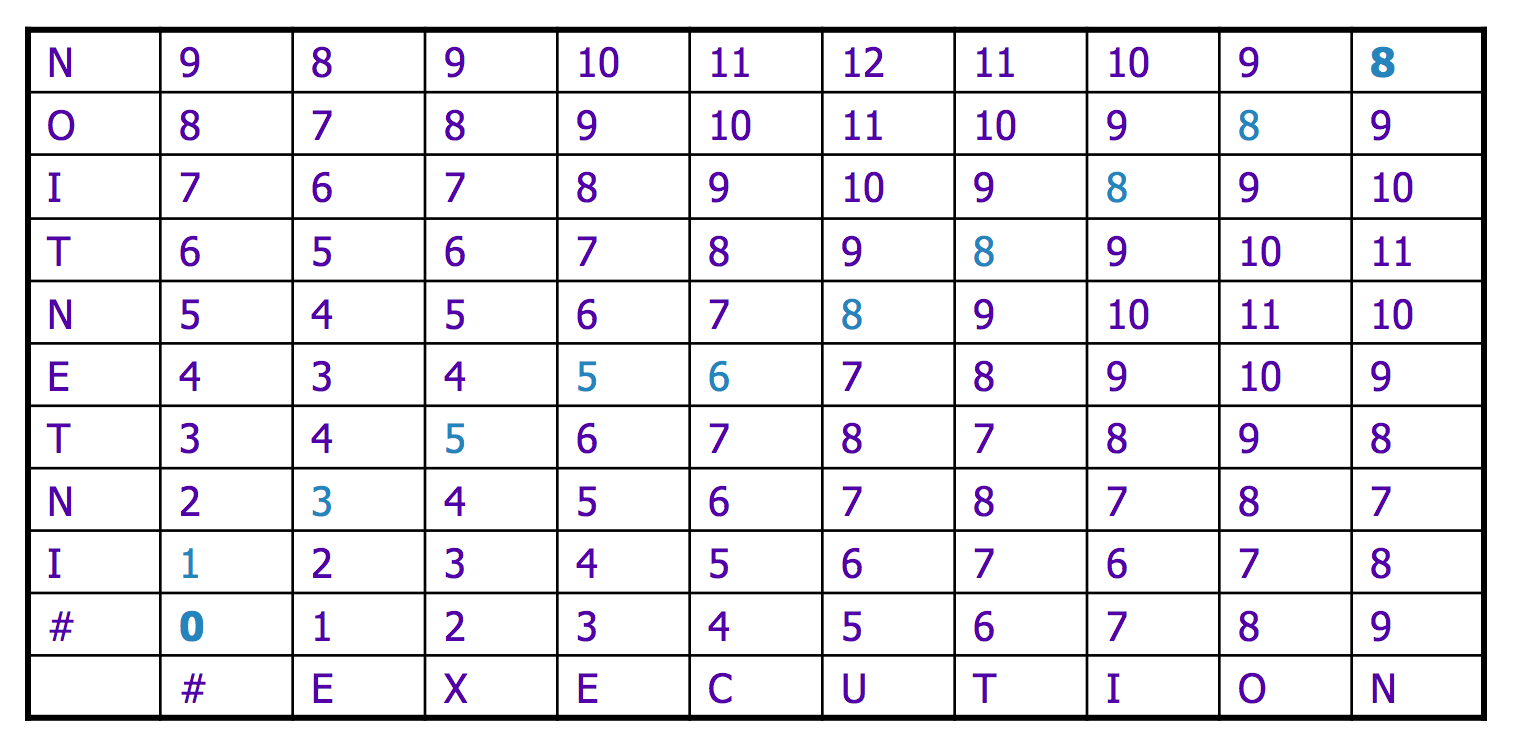
\includegraphics[width=0.5\textwidth]{figures/edit-distance-table.png}
    &
    \vspace{0pt}
    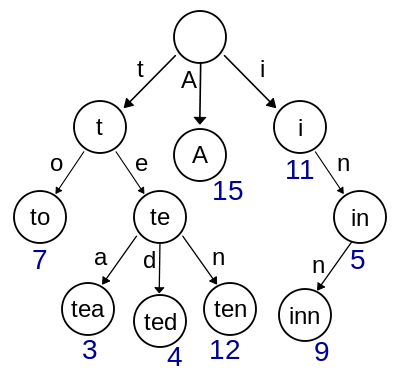
\includegraphics[width=0.5\textwidth]{figures/trie-example.png}
\end{tabular}

\begin{center}
  \textcolor{blue}{\url{https://phiresky.github.io/levenshtein-demo}}
\end{center}

\end{frame}
%------------------------------------------------------------------------------

%------------------------------------------------------------------------------
\section{Model-Based Methods}
%------------------------------------------------------------------------------

%------------------------------------------------------------------------------
\begin{frame}{Pipeline of Models}

\begin{center}
  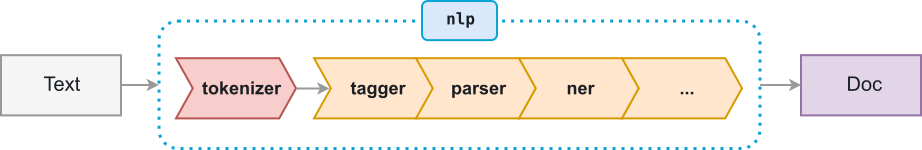
\includegraphics[width=1.0\textwidth]{figures/pipeline.png}
\end{center}

\end{frame}
%------------------------------------------------------------------------------


\end{document}
